\documentclass[conference]{IEEEtran}
\usepackage{authblk}
\usepackage{graphicx}
\graphicspath{ {./images/} }
%\usepackage{babel}
\usepackage{amsmath, amsfonts}

\usepackage[nottoc]{tocbibind}
\usepackage[european resistors, straightvoltages]{circuitikz}

\author[1]{Jay Piamjariyakul}
\author[2]{Felix Kong}
\affil[1]{Undergraduate, Department of Electrical \& Electronic Engineering, University of Bristol}
\affil[2]{Department of Mechanical Engineering, University of Bristol}
\title{Generating Electricity with Footsteps: Analysis of the Proposed Mechanism}

\renewcommand\IEEEkeywordsname{Keywords}
\newcommand{\figref}[1]{\figurename~\ref{#1}}
\newcommand{\compref}[1]{Component~\ref{#1}}
\newcommand{\stepref}[1]{Step~\ref{#1}}

\begin{document}

\maketitle
\begin{abstract}
This document examines the plausibility \& efficiency of generating power via footsteps, which could be used on pavements to generate electricity used for various purposes, depending on the user's preferences.
\end{abstract}

% \begin{IEEEkeywords}
%     Component (comp.)
% \end{IEEEkeywords}
 
% \section{Preamble}
% The application of utilising footsteps to generate electricity adapts the mechanisms of a dynamo (which generates electricity from mechanical torque input) and that of a pressure plate (akin to those used in vintage spinning-top toys). Its applications, theoretically, could be used to alleviate lack of electricity in remote regions (given a large amount of foot-based commuting) or help local businesses collect data in regards to visitors/browsers \& determine their best course of business action.

\section{Mechanism Proposal}
The proposed mechanism to generate electricity is comprised of multiple stages, and such operate in unison to provide the output voltage at the output stage.

\subsection{Components Analysis}
The mechanism itself involves a button/plate that, when pressed, would push a spiral down an entry point, compressing a spring. When such button/plate (thus, the spring) is released, the spiral is released to its initial position, in turn spinning the flywheel disc/gear that such spiral is fixed to, causing such to move in a rotational manner.

\begin{figure}[ht]
    \centering
    \caption{Diagram of proposed mechanism to generate electricity from footsteps}
    \label{fig:mech_wlabel}
    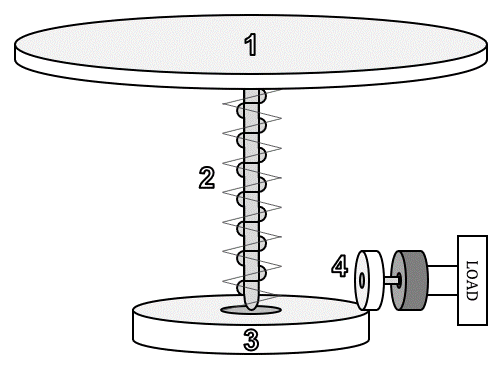
\includegraphics[width=\linewidth]{mech_wlabel.png}
\end{figure}

Such mechanism is shown in \figref{fig:mech_wlabel} and is comprised of the following components (refer to labels on \figref{fig:mech_wlabel}):
\begin{enumerate}
    \item\label{item:comp:plate} Plate which individual steps onto - such is supported by a compression spring
    \item\label{item:comp:spiral} Spiral rod which inserts into \compref{item:comp:flywheel}'s axle - such is attached to \compref{item:comp:plate}
    \item\label{item:comp:flywheel} Flywheel which \compref{item:comp:spiral} inserts into via an opening fitting the size of the spiral's rectangular body
    \item\label{item:comp:motor} Motor with additional gears connected to \compref{item:comp:flywheel}, where such is repurposed as a generator; such gears may include transmission stages
\end{enumerate}

\subsection{Operations of Mechanism}
The mechanism is intended to operate per the following procedures (refer to labels on \figref{fig:mech_wlabel}):
\begin{enumerate}
    \item\label{item:op:stepdn} One steps onto \compref{item:comp:plate}, pushing \compref{item:comp:spiral} downwards \& compressing the support spring
    \item\label{item:op:spiraldn} \compref{item:comp:spiral} moving downwards passes through slot in \compref{item:comp:flywheel}
    \item\label{item:op:stepup} One steps away from \compref{item:comp:plate}, resulting in the spring being released; such results in \compref{item:comp:spiral} moving upwards to its original position
    \item\label{item:op:spin} \compref{item:comp:spiral} moving upwards now results in \compref{item:comp:flywheel} rotating, causing \compref{item:comp:motor}'s axle to also be rotated (due to the gear connection)
    \item\label{item:op:induce} The rotation of \compref{item:comp:motor}'s axle results in EMF being generated at its output
\end{enumerate}

One can surmise that power from \textbf{linear motion} (due to Steps \ref{item:op:stepdn} and \ref{item:op:spiraldn}) is converted to that of \textbf{rotary motion} (given by Step \ref{item:op:spin}), and later converted via \textbf{induction} (per Step \ref{item:op:induce}).

% ------------------------------
% ------------------------------

% \subsection{Electromagnetic Induction}
% One recalls Faraday's \textbf{Law of Electromagnetic Induction} (and Lenz' Law)
% \begin{equation}
    % % Use \varepsilon for curly epsilon
    % E = -\frac{d\psi}{dt} \equiv -N\frac{d\phi}{dt} = -N\frac{dBA}{dt}
    % \label{eq:faraday}
% \end{equation}
% where such terms are defined per following:
% \begin{itemize}
    % \item \(E\): \textbf{EMF} generated within coil (V)
    % \item \(\psi\): magnetic \textbf{flux linkage} (Wb Turns)
    % \item \(\phi\): magnetic \textbf{flux} (Wb)
    % \item \(N\): amount of wire turns within a coil (Turns)
    % \item \(B\): magnetic flux density (T)
    % \item \(A\): area of coil (m\(^2\))
% \end{itemize}

% Per \eqref{eq:faraday}, one can observe (with reference to \figref{fig:mechanism_side_wlabel} \& \figref{fig:mechanism_winding_top}) that, as the flywheel (Comp. 5) rotates, the magnetic field generated by the magnets (Comp. 6) only crosses through the wire coil windings, whereas the coil's area does not get altered, and thus is stationary. \eqref{eq:faraday} could thereby be simplified to the following (assuming coil is immute during operation):
% \begin{displaymath}
    % E = -NA\frac{dB}{dt}
% \end{displaymath}

% \subsection{Work Done by Footstep}
% One recalls the general formula of \textbf{power}:
% \begin{equation}
    % \label{eq:power:general}
    % P = \frac{\Delta W}{\Delta t}
% \end{equation}
% where \(P\) is power (measured in Watts), and \(W\) is \textbf{work done} (measured in Joules). Such is applicable in both \textbf{linear} \& \textbf{rotary} motions' stages of the operation.

% One can also recall the formula of \textbf{work done} via \textbf{linear motion}:
% \begin{equation}
    % W = F_L d = (F_f + F_k + F_c)(s-x)
    % \label{eq:work:linear}
% \end{equation}
% where:
% \begin{itemize}
    % \item \(F_L\): \textbf{aggregate force} exerted onto spiral, due to \textbf{linear motion} via person stepping on plate \& spring and damper (N)
    % \item \(F_f\): \textbf{force} exerted by \textbf{person} onto plate (N)
    % \item \(F_k\) \& \(F_c\): \textbf{forces} exerted onto plate by \textbf{spring} and \textbf{damper}, respectively; such forces oppose \(F_f\) \& are in opposite direction to \(F_f\), and thus are negative (N)
    % \item \(d\): maximum possible \textbf{displacement} which spiral/plate can travel downwards (m)
    % \item \(s\): \textbf{distance} between plate \& disc (m)
    % \item \(x\): minimum possible \textbf{displacement} of compressed spring \& damper, assuming both damper and spring compresses to the same displacement (m)
% \end{itemize}

% Similarly, one recalls the formula of \textbf{work done} via \textbf{rotational motion}:
% \begin{equation}
%     W = \tau\theta = F_R r\theta
%     \label{eq:work:rotational}
% \end{equation}
% where:
% \begin{itemize}
%     \item \(\tau\): \textbf{torque} of disc (Nm)
%     \item \(\theta\): \textbf{angle} of rotation of disc (radians)
%     \item \(F_R\): \textbf{force} of rotation tangential to disc, as exerted by spiral (N)
%     \item \(r\): \textbf{radius} of disc (m)
% \end{itemize}

% Per \textbf{conservation of energy}, such \textbf{cannot be created nor destroyed}. Given so, and assuming the following (amongst others):
% \begin{itemize}
%     \item System between linear \& rotational motion operates at 100\% efficiency (not possible in reality)
%     \item There is minimal friction between spiral \& the hole in the disc that such spiral enter into
%     \item Spring \& damper both compress to the same displacement \& returns to its default state
%     \item One stepping on \& off to/from the plate is reminiscent to a step input
% \end{itemize}
% one can equate \eqref{eq:work:linear} and \eqref{eq:work:rotational} to obtain the following:
% \begin{equation}
%     F_L d = F_R r\theta
% \end{equation}


\section{Theory}
% Insert brief intro of section
This section concerns the generator's output characteristics \& how such is linked to the mechanical stage prior. Such refers to \cite{industrial2} in regards to theory \& formula behind such operations.

%Generating electricity from footsteps adapts the fundamental theorems of mechatronics, prominent those involving electromagnetic induction. See \cite{industrial2} for reference.

%\subsection{Electromagnetic Induction}
% One recalls Faraday's \textbf{Law of Electromagnetic Induction} (and Lenz' Law)
% \begin{equation}
%     % Use \varepsilon for curly epsilon
%     \epsilon = -\frac{d\psi}{dt} \equiv -N\frac{d\phi}{dt} = -N\frac{dBA}{dt}
%     \label{eq:faraday}
% \end{equation}
% where such terms are defined per following:
% \begin{itemize}
%     \item \(\epsilon\): \textbf{EMF} generated within coil (V)
%     \item \(\psi\): magnetic \textbf{flux linkage} (Wb Turns)
%     \item \(\phi\): magnetic \textbf{flux} (Wb)
%     \item \(N\): amount of wire turns within a coil (Turns)
%     \item \(B\): magnetic flux density (T)
%     \item \(A\): area of coil (m\(^2\))
% \end{itemize}

% \begin{displaymath}
%     \epsilon = -NA\frac{dB}{dt}
% \end{displaymath}

\subsection{Assumptions of System}
Given reality, that the system will encounter losses, and thus will not be 100\% efficient. This therefore warrants for a number of assumptions to be made, to allow easier calculations \& analyses of the system.
\begin{itemize}
    \item An individual steps onto the slab \& pushes the spiral to its maximum length
    \item There is no friction within the spiral - this results in the flywheel rotation a full revolution per one successful spiral turn
    \item Thermal losses (due to friction or thermal dissipation by the components) are neglegible
    \item The material themselves do not wear down or permanenently change form, thus allowing for sustained usage
    % \item The spiral's upward motion (and thus the flywheel's rotation speed) is constant
    \item The tangential force on the flywheel is fully transferred to the motor/generator
    \item The flywheel and its opening component is regarded as a singular entity
\end{itemize}

\subsection{Known Quantities}
The following electrical values are either known or determined by the chosen equipment.
\begin{itemize}
    \item The \textbf{electromagnetic constant}, \textbf{reluctance} and \textbf{voltage rating} of the motor/generator
    \item Desired voltage at load (i.e. 5V for a rechargeable battery)
\end{itemize}
Similarly, on the mechanical domain one understands that the number of \textbf{spiral turns} is controlled by the spiral rod, and thus is a known value.

\subsection{Generator Output Characteristics}
The generator's output mechanism can be modelled as an equivalent circuit per \figref{circuit:generator}, where the following terms are defined:
\begin{itemize}
    \item $\omega$/$T$: Angular speed \& torque of generator's input axle, dictated by its transmission gear \& stages
    \item $E$: Output EMF of generator
    % \item $\mathcal{R}_a$: Generator reluctance
    \item $R_a$: Generator reluctance
    \item $I_a$/$V_a$: Current \& voltage at load output of generator
\end{itemize}

\begin{figure}[ht]
    \centering
    \label{circuit:generator}
    \caption{Equivalent circuit of generator and its output}
    \begin{circuitikz}
        \draw (0, 0) to[Telmech=G, n=generator] (0, 2) to[short, -*] (1, 2);
        \draw (1, 2) to[R=\text{\(R_a\)}, i=\(I_a\), -o] (4,2);
        \draw (1, 0) to [open, v>=$E$] (1, 2);
        \draw (0, 0) to[short, -*] (1, 0) to[short, -o] (4, 0);
        \draw (4, 0) to [open, v>=$V_{a}$] (4, 2);
        \draw [thick, ->>] (-1.5, 1) -- (generator.left) node[
            midway,above]{$\omega$} node[
                midway,below]{$T$};
    \end{circuitikz}
\end{figure}

Such is governed by the equations given by \eqref{eq:dcmotor}, where $k_e$ is the \textbf{electromagnetic constant} of the motor/generator.
\begin{subequations}
    \label{eq:dcmotor}
    \begin{align}
        T &= k_e I_a
        \label{eq:dcmotor:torque}\\
        E &= k_e \omega
        \label{eq:dcmotor:emf}
    \end{align}
\end{subequations}

Given \figref{circuit:generator} one can surmise the following information given by \eqref{eq:dcmotor}.
\begin{equation}
    \label{eq:circuit}
    \begin{aligned}
        V_a &= E - I_aR_a\\
        &= k_e\omega - \left(\frac{T}{k_e}\right)R_a
    \end{aligned}
\end{equation}
where \(\omega\) and \(T\) are determined by the prior stage, specifically the mechanical input stage.

\subsection{Mechanical Input Characteristics}
% Calculate general omega/tau from spiral rod!!
The following assumptions are to be made in regards to the mechanical stage, to alleviate calculations.
\begin{itemize}
    \item The mass of the flywheel is represented as an arbitrary cylindrical mass of \(M_f\) kg with a radius of \(r_f\) metres
    \item The mass of the slab is, similarly, represented as a point mass of \(M_s\) kg
    \item The spring continuously obeys Hooke's Law
\end{itemize}

\subsubsection{Force Exerted by Spring}
Given the operations of the mechanism, compressing the spring to a certain distance \(x\) from its original position results in a force being exerted outwards (with intent of returning to its original shape), and thus obeys Hooke's Law per \eqref{eq:hooke}.
\begin{equation}
    \label{eq:hooke}
    F = -kx
\end{equation}
where \(x\) is the total distance compressed by the spring.

% Due to Conservation of Energy \& the assumptions made prior, it can be surmised that the elastic potential energy of the spring is fully transferred to the next stage, per \eqref{eq:epe} as derived from \eqref{eq:hooke}.
% \begin{equation}
%     \label{eq:epe}
%     \text{\textit{Work Done}} = \Delta PE = \frac{1}{2}kx^2
% \end{equation}

\subsubsection{Tangential Force of Flywheel}
As the spiral rod passes through the opening gap inside the flywheel, force is exerted by the spiral rod incident to the opening's sides (assumed here to be point incidents). It can be assumed that, during upward motion, the flywheel and the spiral port moves as a single object, and thus is abstracted as a single entity in the flywheel itself.

% Work done by such action is then given per \eqref{eq:spiral}.
% \begin{equation}
%     \label{eq:spiral}
%     \text{\textit{Work Done}} = F_f r\theta \equiv T\theta
% \end{equation}
% where \(r\) is the radius of the flywheel, \(F_f\) is (assumedly point) tangential force exerted onto the flywheel, and \(\theta\) is the total angle which flywheel travels (in radians), given to be \(2\pi N\) per \(N\) spiral turns.

% Equating \eqref{eq:epe} and \eqref{eq:spiral} (per Conservation of Energy and the full-efficiency assumption) results in an expression for force.
% \begin{equation*}
%     \frac{1}{2}kx^2 = 2\pi NFr = 2\pi NF_{edge}d
% \end{equation*}

% In the case of the equated expression, one could then obtain the tangential force exerted at the edge of the flywheel's body, per \eqref{eq:f_edge}.
% \begin{equation}
%     \label{eq:f_edge}
%     \frac{1}{2}kx^2 = 2\pi NF_{edge}d
% \end{equation}

The expression for tangential force on the flywheel is given per \eqref{eq:flywheel}, where  
\begin{equation}
    \label{eq:flywheel}
    F = T\omega \equiv \frac{T\theta}{t}
\end{equation}
where \(F\) is (assumedly point) tangential force exerted onto the flywheel, and \(\omega\) is the angular velocity of the flywheel. In addition, \(\theta\) is the total angle which flywheel travels (in radians), and \(t\) is the time at which the spring reverts to its original length, and is variable by the person stepping onto the slab.

It is to be noted that \(\theta\) is given to be \(2\pi Q\) per \(q\) spiral turns.


\subsubsection{Equating}
Provided that \eqref{eq:hooke} and \eqref{eq:flywheel} equate, one could obtain the expression for the raw torque obtained at the flywheel's edge, per \eqref{eq:equate}.
\begin{equation}
    \label{eq:equate}
    T = \frac{-tkx}{2\pi Q}
\end{equation}

However, the motor itself is to be connected via a buffer gear, which would allow one to vary the torque and angular velocity of the motor.

\subsection{Mechanical Output Characteristics}
Since connecting the flywheel and the motor together results in the same tangential force, one could equate \(F\) and obtain an expression in terms of torque \& angular velocity of the motor, where such are \(T_m\) and \(\omega_m\), respectively.

\begin{equation*}
    F = T_m \omega_m
\end{equation*}

Given that the flywheel's attributed are controlled variables, one could only change the motor's gear and, provided the attributes of the flywheel's gear, could determine the ratio of turns between such gear connections.

\begin{equation*}
    \Gamma = \frac{N_{motor}}{N_{flywheel}}
\end{equation*}

And thus, one could then obtain the expression for the motor's torque \& angular velocity in terms of the flywheel's.

\begin{equation}
    \label{eq:ratio}
    F = T_{motor}\omega_{motor} = (T\Gamma)\left(\frac{\omega}{\Gamma}\right)
\end{equation}

Per \eqref{eq:ratio} one could observe that a decrease in the number of gear 'teeth' on the motor's, such reduces the coefficient, and thus reduces the motor's torque while increasing its angular velocity. Vice versa applies.

Sufficient information has been provided to return to \eqref{eq:dcmotor:emf}; now that one has obtained the motor's characteristics, one could then equate such to those that one has explored prior as follows.

\begin{align*}
    V_a &= k_e(\omega_{f} \Gamma) - \left(\frac{T_{f}\Gamma}{k_e}\right)R_a \\
    &=  k_e\left(\frac{2\pi Q}{t} \Gamma\right) - \left(\frac{1}{k_e}\right)\left(\frac{-tkx}{2\pi Q}\Gamma\right)R_a
\end{align*}

Given this, the only independent variable (provided components are static, thus its values fixed) to determine the output voltage of the mechanism is the time duration taken to reload the spring mechanism back to its original position.


% \begin{subequations}
%     For one spiral turn
%     \begin{align}
%         \omega &= \frac{n 2\pi}{\Delta t} = \frac{2\pi}{\Delta t}
%     \end{align}
% \end{subequations}


% \section{Simulation}
% One utilises MATLAB's SimScape to simulate such mechanisms, and is comprised of three stages.
% % Check if intro line is necessary and/or needs amendment!

% \subsection{Schematic Diagram}

% ------------------------------
% ------------------------------

\medskip
\bibliographystyle{IEEEtran}
\bibliography{references}
\end{document}